\documentclass[11pt,xcolor={usenames,dvipsnames,svgnames},compress]{beamer}

\usepackage{booktabs}
\usepackage{multirow}
\usepackage{dcolumn}
\usepackage{colortbl}
\usepackage{xcolor}
\usepackage{hyperref}
\usepackage{amsmath}
\usepackage{wrapfig}
\usepackage{algorithm}
\usepackage[noend]{algpseudocode} 
\usepackage{pifont}
\usepackage{listings}
\usepackage[style=authoryear-icomp,backend=bibtex, mincitenames=2, maxcitenames=2]{biblatex}
\usepackage{marvosym}
\usepackage{mathtools}
\usepackage{array}
\usepackage[export]{adjustbox}
\usepackage{bm}
\usepackage{dsfont}
\usepackage{subcaption}

\usepackage[font=scriptsize]{caption}
      
\lstdefinelanguage{json}{
    basicstyle=\fontsize{9}{11}\ttfamily,
    numbers=left,
    numberstyle=\scriptsize,
    stepnumber=1,
    numbersep=8pt,
    showstringspaces=false,
    breaklines=true,
    frame=lines,
    backgroundcolor=\color{background},
    literate=
      {:}{{{\color{punct}{:}}}}{1}
      {",}{"{{\color{punct}{,}}}}{1}
      {\{}{{{\color{delim}{\{}}}}{1}
      {\}}{{{\color{delim}{\}}}}}{1}
      {[}{{{\color{delim}{[}}}}{1}
      {]}{{{\color{delim}{]}}}}{1}}

\colorlet{punct}{red!60!black}
\definecolor{background}{HTML}{EEEEEE}
\definecolor{delim}{RGB}{20,105,176}
\colorlet{numb}{magenta!60!black}

\definecolor{untractable_red}{RGB}{209, 25, 25}
\definecolor{tractable_green}{RGB}{0, 153, 51}

\newcommand{\argmax}{\operatornamewithlimits{argmax}}
\newcommand{\argmin}{\operatornamewithlimits{argmin}}
\newcommand{\nodeset}[1]{\bm{\mathsf{#1}}}
\newcommand{\cbar}{\,|\,}

\newcolumntype{R}[2]{
  >{\adjustbox{angle=#1,lap=\width-(#2)}\bgroup}
  l
  <{\egroup}
}

\newcommand*\rot{\multicolumn{1}{R{45}{1em}}}

\definecolor{lacamgreen} {RGB} {72, 175, 115}
\definecolor{lacamlilac} {RGB} {107,93,153}
\definecolor{lacamlilac2} {RGB} {93, 109, 152}
\definecolor{lacamlightlilac} {RGB} {174, 166, 201}
\definecolor{lacamdarklilac} {RGB} {51, 10, 102}
\definecolor{lacamgold} {RGB} {255, 87, 0}
\definecolor{lacamdarklilac5} {RGB} {51, 10, 102}
\definecolor{lacamgold5} {RGB} {255, 87, 0}
\definecolor{violet} {RGB} {119, 111, 178}
\definecolor{petroil2} {RGB} {36, 165, 175}
\definecolor{petroil4} {RGB} {30, 132, 149}
\definecolor{petroil6} {RGB} {23, 101, 115}
\definecolor{gold2} {RGB} {255, 130, 0}
\definecolor{gold4} {RGB} {250, 100, 0}
\definecolor{gold6} {RGB} {245, 90, 0}
\definecolor{darkred} {HTML} {67000C}

\definecolor{tomato0} {HTML} {EF9A9A}
\definecolor{tomato1} {HTML} {F44336}
\definecolor{tomato2} {HTML} {E53935}
\definecolor{tomato3} {HTML} {D32F2F}
\definecolor{tomato4} {HTML} {C62828}
\definecolor{tomato5} {HTML} {B71C1C}


\definecolor{peas1} {HTML} {009688}
\definecolor{peas2} {HTML} {00897B}
\definecolor{peas3} {HTML} {00796B}
\definecolor{peas4} {HTML} {00695C}
\definecolor{peas5} {HTML} {004D40}

\definecolor{bgrey0} {HTML} {78909C}
\definecolor{bgrey1} {HTML} {607D8B}
\definecolor{bgrey2} {HTML} {546E7A}
\definecolor{bgrey3} {HTML} {455A64}
\definecolor{bgrey4} {HTML} {37474F}
\definecolor{bgrey5} {HTML} {263238}

\definecolor{olive0} {HTML} {C5E1A5}
\definecolor{olive1} {HTML} {AED581}
\definecolor{olive2} {HTML} {9CCC65}
\definecolor{olive3} {HTML} {8BC34A}
\definecolor{olive4} {HTML} {7CB342}
\definecolor{olive5} {HTML} {689F38}

\definecolor{pink0} {HTML} {FCE4EC}
\definecolor{pink1} {HTML} {F8BBD0}
\definecolor{pink2} {HTML} {F48FB1}
\definecolor{pink3} {HTML} {F06292}
\definecolor{pink4} {HTML} {EC407A}
\definecolor{pink5} {HTML} {FF80AB}

\definecolor{brown0} {HTML} {D7CCC8}
\definecolor{brown1} {HTML} {BCAAA4}
\definecolor{brown2} {HTML} {A1887F}
\definecolor{brown3} {HTML} {8D6E63}
\definecolor{brown4} {HTML} {795548}
\definecolor{brown5} {HTML} {6D4C41}
\definecolor{brown6} {HTML} {5D4037}

\definecolor{yellow0} {HTML} {CDDC39}
\definecolor{yellow1} {HTML} {9E9D24}
\definecolor{yellow3} {HTML} {FFBD2A}
\definecolor{yellow4} {HTML} {FFB000}
\definecolor{yellow5} {HTML} {FFD600}

\AtEveryCite{\color{violet}\bf}

\newcommand{\highlight}[2][yellow]{\mathchoice%
  {\colorbox{#1}{\textcolor{white}{$\displaystyle{#2}$}}}
  {\colorbox{#1}{\textcolor{white}{$\textstyle{#2}$}}}
  {\colorbox{#1}{\textcolor{white}{$\scriptstyle{#2}$}}}
  {\colorbox{#1}{\textcolor{white}{$\scriptscriptstyle{#2}$}}}}

\newcommand{\highlighttext}[2][yellow]{{\colorbox{#1}{\textcolor{white}{#2}}}}

\usetheme{enziteto}

\setbeamertemplate{headline}{}

\newcommand*\samethanks[1][\value{footnote}]{\footnotemark[#1]}

\makeatletter
\renewcommand*{\@fnsymbol}[1]{\ensuremath{\ifcase#1\or $\Yinyang$\or \dagger\or \ddagger\or
    \mathsection\or \mathparagraph\or \|\or **\or \dagger\dagger
    \or \ddagger\ddagger \else\@ctrerr\fi}}
\makeatother

\setbeamerfont{footnote}{size=\scriptsize}
\newcommand{\customcite}[1]{\footnote{\tiny \citeauthor{#1}, \citetitle{#1}, \citeyear{#1}}}
\newcommand{\customcitenomark}[1]{\footnotenomarkleft{\tiny
    \citeauthor{#1}, \citetitle{#1}, \citeyear{#1}}}
\newcommand{\customcitetext}[1]{\footnotenomarkleft{\tiny \citeauthor{#1}, \citetitle{#1}, \citeyear{#1}}}

\definecolor{untractable_red}{RGB}{209, 25, 25}
\definecolor{tractable_green}{RGB}{0, 153, 51}

\newcommand{\cmark}{\ding{51}}
\newcommand{\xmark}{\ding{55}}

\newcommand{\plusbullet}{\raisebox{\custombulletheight}{\hbox{\tiny\textcolor{lacamlilac}{$\boldsymbol{\oplus}$}}\hspace{-2pt}}}

\setbeamertemplate{itemize item}{\raisebox{.21ex}{\hbox{\tiny\textcolor{lacamlilac}{$\boldsymbol{\oplus}$}}\hspace{-2pt}}}
\setbeamertemplate{itemize subitem}{\raise .2ex\hbox{\tiny\textcolor{lacamlilac}{$\boldsymbol{\otimes}$}}\hspace{-3pt}}
\setbeamertemplate{itemize subsubitem}{\textcolor{lacamlilac}{$\oplus$}}
\setbeamertemplate{bibliography item}{\hspace{10pt}\raise .2ex\hbox{\t, 10ptiny\textcolor{lacamlilac}{$\boldsymbol{\oplus}$}}}

\setbeamertemplate{bibliography item}{\hspace{10pt}\raise
  .2ex\hbox{\textcolor{lacamlilac}{$\boldsymbol{\oplus}$}}}

\begin{document}

\newlength{\custombulletheight}
\setlength{\custombulletheight}{\dimexpr0.5\ht1-0.5\ht2}

\title{Analisi di Social Media per la \\ Scoperta di Pattern di Interazione}
\author{\textit{Relatori}: \\ dr. Corrado Loglisci \\ prof. Donato Malerba \\ [1.5ex] 
\textit{Correlatore}: \\ dott. Angelo Impedovo 
\begin{flushright}\textit{Laureando}: \\ Donato Meoli \end{flushright}}
\subtitle{Tesi di Laurea in Metodi Avanzati di Programmazione}
\date{26 Aprile 2018}
\institute{Università degli Studi di Bari}
\department{Dipartimento di Informatica}
\laboratory{ \hspace{-12.2pt} LACAM}
\group{ \hspace{-11pt} Knowledge Discovery and Data Engineering}
\institutelogo{
\includegraphics[width=25pt]{img/sigillo}}
\lablogo{
\includegraphics[width=20pt]{img/kdde}}

\footnotesize \let\small\footnotesize

{
  \setbeamertemplate{headline}{}
  \setbeamertemplate{footline}{}
  \begin{frame}
    \titlepage
  \end{frame}
}

\begin{frame}
  \frametitle{\textcolor{lacamlilac}{\textbf{\emph{Obiettivo}}}}
  
  \begin{description}
  \item[\textbf{>>}] realizzare strumenti computazionali in grado di modellare comunit{\`a} online
  \item[\textbf{>>}] sintetizzare metodi di analisi che siano in grado di scoprire le interazioni tra i partecipanti
  \end{description}\bigskip
  
\end{frame}

\begin{frame}
  \frametitle{\textcolor{lacamlilac}{\textbf{\emph{Motivazione}}}}
  
  \begin{description}
  \item[\textbf{>>}] recente interesse nel monitoraggio dei partecipanti di piattaforme web attraverso le loro relazioni rispetto ad interessi comuni (es. realizzazione di progetti collaborativi)
  \item[\textbf{>>}] indirizzare questo tipo di informazioni per studi sociali rispetto a tecnologie web o social media
  \end{description}\bigskip  
  
\end{frame}

\begin{frame}
  \frametitle{\textcolor{lacamlilac}{\textbf{\emph{Problematiche}}}}
  
  \begin{description}
    \item[\textbf{>>}] una comunità rappresenta un dominio che evolve nel tempo i cui cambiamenti possono essere molteplici e possono riguardare fattori interni o esterni
  \item[\textbf{>>}] web ricco di User Generated Content (UGC) di tipo non strutturato (es. contenuti di Twitter, StackOverflow, Wikipedia, Reddit, ecc.)
  \item[\textbf{>>}] ambiguit{\`a} relativa alle informazioni prodotte in linguaggio naturale
  \item[\textbf{>>}] contenuti sintetici, soggetti ad errori ortografici e a linguaggio web (es. lol, asd, ecc.)
  \end{description}\bigskip
  
\end{frame}

\section{Soluzione Computazionale}
{\setbeamertemplate{headline}{}
  \begin{frame}
    \sectionpage
  \end{frame}
}

\begin{frame}
  \frametitle{\highlighttext[lacamgreen]{\textbf{\emph{Scelta del Modello Computazionale}}}}
  
  \begin{description}
  \item[\textbf{>>}] relazioni non identificate a priori per via delle relazioni sociali che intercorrono tra questi (es. ``follow" o ``amicizia")
  \item[\textbf{>>}] previste relazioni tra gli utenti che sono supportate dagli strumenti tecnologici in uso
  
  \item[\textbf{\Large >>}] rappresentazione a grafo della comunit{\`a} in cui i nodi rappresentano gli utenti e gli archi corrispondono alle relazioni che intercorrono tra di loro
  \end{description}\bigskip
  
\end{frame}

\begin{frame}
  \frametitle{\highlighttext[lacamgreen]{\textbf{\emph{Costruzione del Grafo (1)}}}}
   
   Archi basati su \textcolor{red}{tag sociali}:
   \begin{description}
  \item[\textbf{>> COMMENT\_TO}] l'utente \( b \) commenta il post dell'utente \( a \)
  \item[\textbf{>> REPLY\_TO}] l'utente \( c \) risponde al commento dell'utente \( b \) sotto il post dell'utente \( a \)
  \item[\textbf{>> MENTION\_TO}] l'utente \( s \) menziona l'utente \( m \)
  \end{description} \par

	Archi basati sul \textcolor{red}{contenuto}:
   \begin{description}
  \item[\textbf{>> WRITE\_LEXICALLY\_SIMILAR\_TO}] dovuta alla similarit{\`a} lessicale tra i messaggi contenuti nei post di due utenti coinvolti nella stessa discussione
  \item[\textbf{>> WRITE\_SEMANTICALLY\_SIMILAR\_TO}] dovuta alla similarit{\`a} semantica tra i messaggi contenuti nei post di due utenti coinvolti nella stessa discussione
  \end{description} \par

Negli archi basati sul contenuto la direzionalit{\`a} {\`e} determinata dal timestamp. 

\end{frame}

\begin{frame}
  \frametitle{\highlighttext[lacamgreen]{\textbf{\emph{Costruzione del Grafo (2)}}}}
\begin{figure}\centering
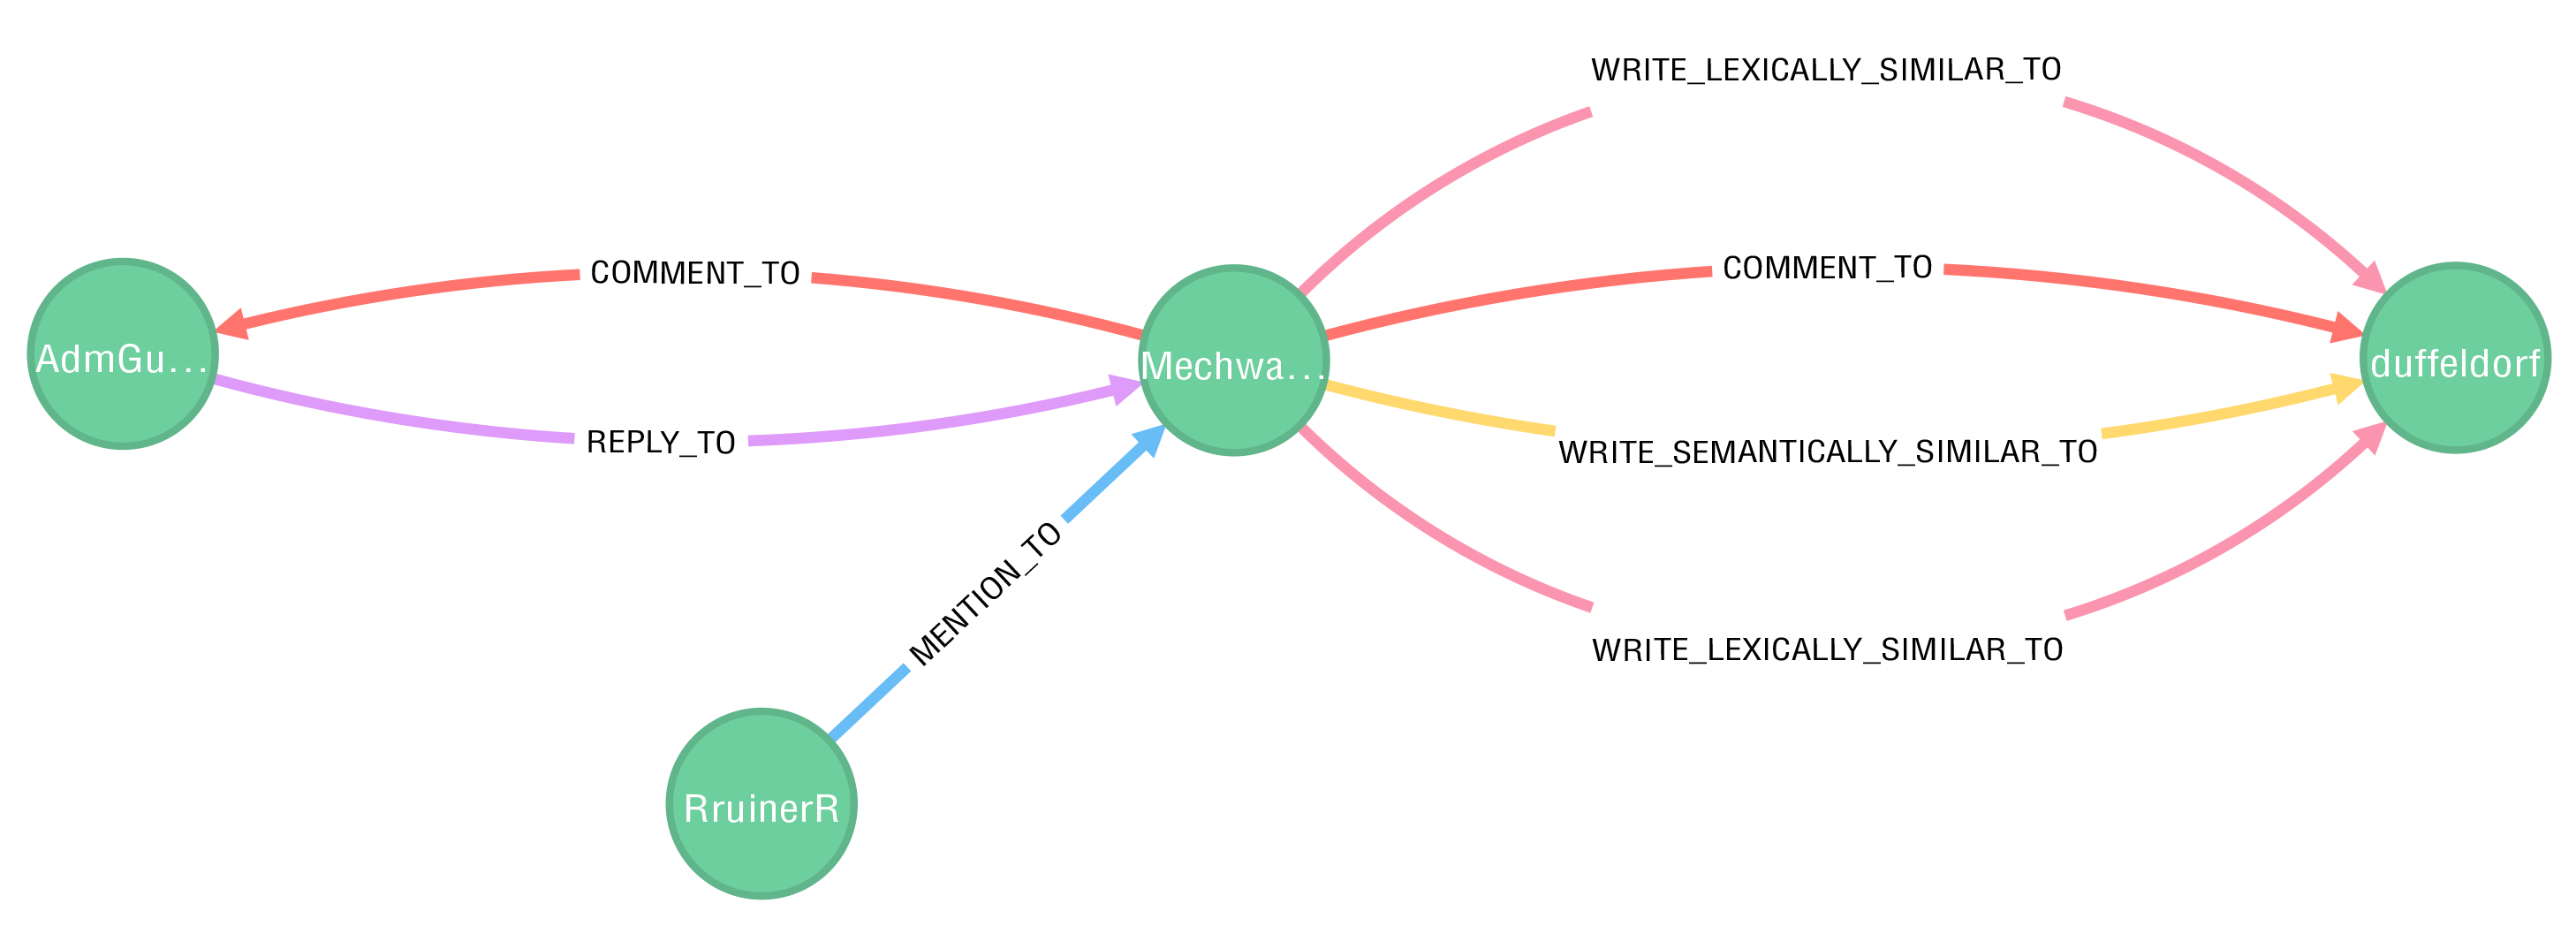
\includegraphics[scale=0.40]{img/graph}
\end{figure}

\end{frame}

\begin{frame}
  \frametitle{\highlighttext[lacamgreen]{\textbf{\emph{Archi Basati sul Contenuto}}}}

  \begin{description}
  \item[\textbf{\highlighttext[tomato0]{\textbf{\emph{>> Similarit{\`a} Lessicale}}}}] \textbf{Lexical Match Algorithm (LMA) \footnote{Fu, Tianjun, Ahmed Abbasi, and Hsinchun Chen. ``A hybrid approach to web forum interactional coherence analysis." Journal of the Association for Information Science and Technology 59.8 (2008): 1195-1209.}}, basato sul Vector Space Model (VSM), considera i messaggi che si presuppone possano essere simili \bigskip
  \item[\textbf{\highlighttext[yellow3]{\textbf{\emph{>> Similarit{\`a} Semantica}}}}] Similarit{\`a} di \textbf{Lin} \footnote{Lin, Dekang. ``An information-theoretic definition of similarity." Icml. Vol. 98. No. 1998. 1998.} pesata con i TF-IDF \footnote{Term Frequency - Inverse Document Frequency} per far si che i termini pi{\`u} frequenti, e quindi semanticamente meno discriminanti, abbiano un'incidenza minore sul valore di similarit{\`a} finale
  \end{description} \bigskip

\end{frame}

\section{Scoperta di Interazioni}
{\setbeamertemplate{headline}{}
  \begin{frame}
    \sectionpage
  \end{frame}
}
 
\begin{frame}
  \frametitle{\highlighttext[peas3]{\textbf{\emph{Analisi di Grafi Temporali}}}}
  
   \begin{description}
  \item[\textbf{>>}] interazioni scoperte in base a densit{\`a} e frequenza
  \item[\textbf{>>}] analisi del grafo per \textcolor{red}{time-point} al fine di scoprire interazioni tra gli utenti basate su frequenza
    \item[\textbf{>>}] analisi di \textcolor{red}{time-windows} di ampiezza incrementale in forma di grafi \textit{cumulativi}, rispetto a quelli di ogni time-point presente nella stessa, al fine di scoprire il ruolo degli utenti e le interazioni tra di essi basate su densit{\`a}
  \end{description} 

\begin{figure}\centering
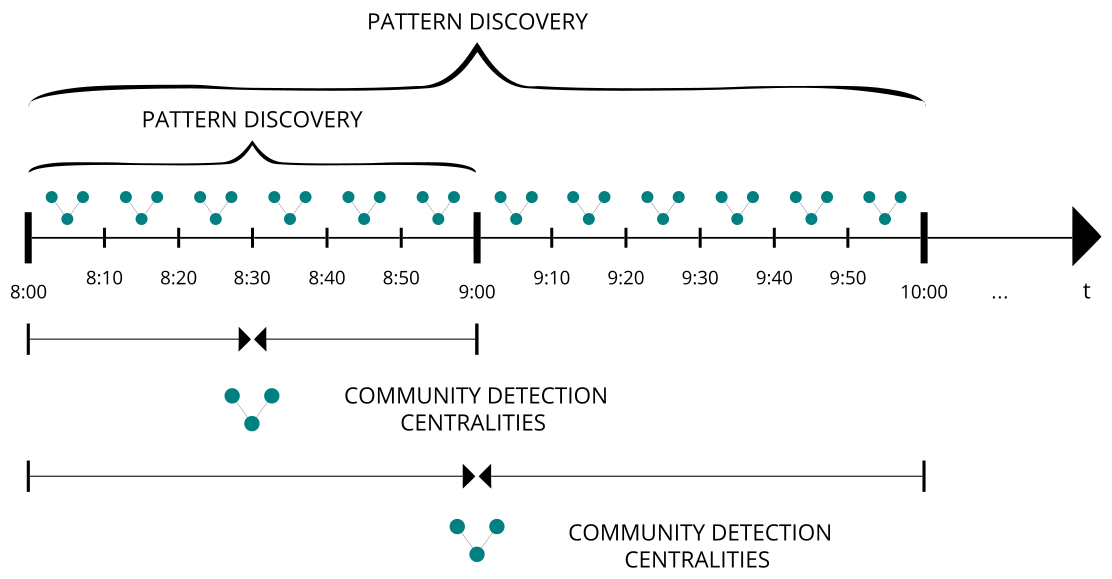
\includegraphics[scale=0.20]{img/temp-graph}
\end{figure} 
 
\end{frame}
 
\begin{frame}
\frametitle{\highlighttext[peas3]{\textbf{\emph{Ruolo dell'Utente: Indicatori di Centralit{\`a}}}}}

  Indicatori nodali definiti in teoria dei grafi:   
  
 \begin{description}
  \item[\textbf{>> Centralit{\`a} ``Degree''}] numero degli archi in cui un nodo {\`e} coinvolto facendo distinzione tra quelli in entrata (``in-degree") e quelli in uscita (``out-degree") al fine di mettere in evidenza il ruolo degli utenti come attrattori o mittenti \par
  \item[\textbf{>> Centralit{\`a} ``Betweenness"}] basata sul calcolo dei cammini minimi, utile per trovare i nodi che fungono da tramite da una parte all'altra del grafo \par
  \item[\textbf{>> Centralit{\`a} PageRank}] determina una stima dell'importanza del nodo all'interno del grafo
  \end{description}\bigskip
 
\end{frame}

\begin{frame}
\frametitle{\highlighttext[peas3]{\textbf{\emph{Interazioni Basate su Densit{\`a}:}}} \\ \highlighttext[peas3]{\textbf{\emph{Scoperta di Comunit{\`a}}}}}
  
   \begin{description}
  \item[\textbf{>>}] un grafo ha una struttura di comunit{\`a} se i suoi nodi possono essere raggruppati in modo tale che quelli di ogni comunit{\`a} siano \textit{densamente} connessi internamente ed abbiano connessioni pi{\`u} \textit{sparse} tra di loro
  \item[\textbf{>>}] metodo di \textbf{Louvain} \footnote{Blondel, Vincent D., et al. ``Fast unfolding of communities in large networks." Journal of statistical mechanics: theory and experiment 2008.10 (2008): P10008.} basato sulla massimizzazione della \textit{modularit{\`a}} di una partizione: funzione euristica che misura la bont{\`a} di una comunit{\`a} ossia la densit{\`a} dei collegamenti all'interno di essa rispetto ai collegamenti tra le comunit{\`a}
  \end{description}\bigskip
  
\end{frame}

\begin{frame}
  \frametitle{\highlighttext[peas3]{\textbf{\emph{Interazioni Basate su Frequenza:}}} \\ \highlighttext[peas3]{\textbf{\emph{Scoperta di Sottografi Frequenti}}}}

\begin{description}
  \item[\textbf{>>}] indagare la presenza di sottografi frequenti rispetto ad una time-window, a partire dai sottografi dei singoli time-point contenuti in essa
  \item[\textbf{>>}] algoritmo \textbf{ECLAT} \footnote{Zaki, Mohammed Javeed, et al. ``New Algorithms for Fast Discovery of Association Rules." KDD. Vol. 97. 1997.} basato su intersezioni insiemistiche e proprit{\`a} connesse per la scoperta di sottografi frequenti
  \end{description}\bigskip  
  
\end{frame}  
   
\section{Esperimenti}
{\setbeamertemplate{headline}{}
  \begin{frame}
    \sectionpage
  \end{frame}
}   

\begin{frame}
  \frametitle{\highlighttext[tomato1]{\textbf{\emph{Dataset: Reddit, Novembre 2017}}}}
  Filtraggio preventivo per garantire un dataset formato da utenti particolarmente attivi e da discussions e commenti semanticamente significativi.

  \begin{description}
  \item[\textbf{>> Submissions}] per cui il numero di commenti {\`e} maggiore di 8 e la lunghezza del selftext {\`e} maggiore di 168 caratteri
  \item[\textbf{>> Commenti}] per cui la lunghezza del body {\`e} maggiore di 170 caratteri
  \item[\textbf{>> Redditors}] che hanno scritto pi{\`u} di 20 discussions e commenti
  \item[\textbf{>> Subreddits}] i 20 migliori tra quelli per cui il numero di discussions che vi appartengono, in seguito al filtraggio definito dai criteri precedenti, risulti maggiore di 77
  \end{description}\par
  
\begin{figure}\centering

\includegraphics[scale=0.12]{img/reddit}
\end{figure}

\end{frame}  

\begin{frame}
  \frametitle{\highlighttext[tomato1]{\textbf{\emph{Setting Sperimentale e Risultati Quantitativi}}}}
  
     \begin{description}
  \item[\textbf{>> time-windows}]  da 1 giorno
  \item[\textbf{>> time-points}] da 3 ore 
  \end{description} \bigskip 
  
  \begin{center}
  \begin{tabular}{| l | c | c | c |}
    \hline
    {} & \multicolumn{2}{| c |}{sottografi} & {comunit{\'a}} \\ \hline
    {} & 2 utenti & 3 utenti & {} \\ \hline
    $\mu$ & 1.476,83 & 3.126,76 & 87,97 \\ \hline
    $\sigma$ & 2.919,28 & 6.391,88 & 150,60 \\ 
    \hline
  \end{tabular}
\end{center}  

\end{frame} 

\begin{frame}[fragile]
  \frametitle{\highlighttext[tomato1]{\textbf{\emph{Risultati Qualitativi (1)}}}}
  
Redditor \url{"D2TournamentThreads"}, prima time-window analizzata (01-02/11):  
  
\begin{lstlisting}[language=json]
{
  "name": "D2TournamentThreads",
  "inDegree": 4,
  "outDegree": 2,
  "betweenness": 4.0,
  "pageRank": 0.39862500000000006,
  "frequentSubgraphs": [
    "{e(D2TournamentThreads, MENTION_TO, 3947977282),
      e(D2TournamentThreads, MENTION_TO, 5874306284)}"
  ]
}
\end{lstlisting}
  
\end{frame} 

\begin{frame}[fragile]
  \frametitle{\highlighttext[tomato1]{\textbf{\emph{Risultati Qualitativi (2)}}}}
  
Redditor \url{"D2TournamentThreads"}, ultima time-window analizzata (29-30/11):    
  
\begin{lstlisting}[language=json]
{
  "name": "D2TournamentThreads",
  "inDegree": 497,
  "outDegree": 21,
  "betweenness": 80639.51145093024,
  "pageRank": 46.710466999999994,
  "frequentSubgraphs": [
    "{e(D2TournamentThreads, MENTION_TO, 1107888450),
      e(D2TournamentThreads, MENTION_TO, 5695452105)}",
    "{e(D2TournamentThreads, COMMENT_TO, 1107888450),
      e(D2TournamentThreads, COMMENT_TO, 5874306284)}",
    "{e(D2TournamentThreads, REPLY_TO, 1107888450),
      e(D2TournamentThreads, REPLY_TO, 5695452105),
      e(D2TournamentThreads, REPLY_TO, 5874306284)}"
      . . .
  ]
}
\end{lstlisting}
  
\end{frame} 

\begin{frame}
  \frametitle{\textcolor{lacamlilac}{\textbf{\emph{Conclusioni}}}}
  
  \begin{description}
  \item[\textbf{>>}] studio di comunit{\'a} online a partire dalla messaggistica intercorsa tra i partecipanti
  \item[\textbf{>>}] soluzione computazionale basata su un modello relazionale e tecniche di data mining
  \end{description} \bigskip 
  
\end{frame}

\begin{frame}
  \frametitle{\textcolor{lacamlilac}{\textbf{\emph{Sviluppi Futuri}}}}
  
  \begin{description}
  \item[\textbf{>>}] sperimentazione su altri social media
  \item[\textbf{>>}] aggiunta di archi basati sulla similarit{\'a} emozionale dei partecipanti in relazione al contenuto dei messaggi scambiati
  \item[\textbf{>>}] analisi delle evoluzioni delle interazioni tra i partecipanti 
  \end{description} \bigskip
  
\end{frame}

\begin{center}
\section{\huge{Grazie per l'Attenzione}}
{\setbeamertemplate{headline}{}
  \begin{frame}
    \sectionpage 
  \end{frame}
}   
\end{center}

\end{document}
